\documentclass[10pt,twocolumn,letterpaper]{article}

\usepackage{cvpr}
\usepackage[utf8]{inputenc}
\usepackage{gensymb}
\usepackage{graphicx}
\usepackage{mathtools}
\graphicspath{ {report2-imgs/} }
\usepackage{float}
\PassOptionsToPackage{hyphens}{url}\usepackage{hyperref}

\cvprfinalcopy
\def\cvprPaperID{a1700831}


% begin of document
\begin{document}
\title{Assignment 2 - Method for Face Detection by Viola and Jones}
\author{Yuanzhong Xia\\
University of Adelaide\\
SA, Australia\\
{\tt\small a1700831@student.adelaide.edu.au}
}
\maketitle

% abstract
\begin{abstract}
This assignment 2 report describes the Viola and Jones's method \cite{origin} which can detect a specified object very rapidly.
Their method uses a machine learning method named AdaBoost \cite{adaboost} to both select important features and classify the images.
The challenge is the potential feature space is very large, therefore, it is very necessary to discard the useless features to reduce the computational cost.
To solve this problem, a cascade structure of the final classifier is introduced. It can reduce a majority of features in each layer,
and most classifiers are applied only on the useful features to provide more accurate prediction result.

The related codes are in Python 3, using the OpenCV C++ binding for Python,
and it contains my testing codes to evaluate my hypothesis and program performance.
\end{abstract}


\section{The Problem}
The problem is to detect face(s) from an input image, and output the image with each face marked with a bounding box.
Although it looks very simple and we don't need to recognize a specific face, the challenge is to detect all the faces in real time.
Because in any normal image, there are so many possible positions and sizes for a single face,
and it's impossible to try every sub-window of them due to the huge computational cost.

Moreover, an input image is not always predictable. The head direction, face integrity, environmental light brightness,
camera features, image quality, etc. can often bring issues to the face detection problem.
And to simplify the problem, the method from Viola and Jones demonstrates with a frontal face detection system,
which means the effects of ``head direction'' and ``face integrity'' are ignored.


\section{Background} \label{sec:bg}
Face detection has been a typical experiment in object detection area.
Lots of researchers use face detection to examine their object detection methods.
Before Viola and Jones's work, there were already some existing object detection algorithms applied on face detection.

Amit et al. came out with an object detection algorithm in 1997 \cite{joint}, which is based on tree-based shape features.
The shapes are generated by a BFS-like procedure, and the generated shapes are applied into training images.
Then, an enumeration procedure is taken to find the potential geometric relationships, and the final model is the set of relationships.
By applying the model into testing images, the images can be classified.

Roth et al. created an snow-based face detecting algorithm \cite{snowbased} which use
% TODO

Rowley et al. used neural network to do face detection \cite{nnbased}.
% TODO

Schneiderman et al. used a statistical method for face detection \cite{stat3d}.
% TODO

Sung et al. used an example-based learning method \cite{examplebased}.
% TODO: describe the competing approaches to the problem


\section{Viola and Jones's Method}
Viola and Jones's method is designed to be applied in any object detection case, and the detection speed is extremely fast around the publish year (2001).
In the paper, all details of the algorithm are demonstrated in doing face detection.
Comparing to other face detection methods whose speeds are faster than Viola and Jones's method,
those methods' speeds are based on checking image difference between the adjacent frames,
while Viola and Jones's method in the demo proceeds each frame independently which means it can achieve even higher speed using the frame difference.

The method has three main steps:
\begin{enumerate}
    \item Compute integral image and Harr-like features;
    \item In each cascading stage:
          \begin{enumerate}
              \item Select the important features, discard the rest features;
              \item Update the accumulated classifier by adjusting thresholds (weights of selected features) using AdaBoost;
          \end{enumerate}
\end{enumerate}

The final cascading classifiers are the final model, classifiers in each layer can reject most features.
Therefore, the computing time gets reduced significantly.

\subsection{Computing features} \label{sec:cf}
The features used in this paper are Haar basis functions motivated by Papageorgiou et al.'s work. (mentioned in Section \ref{sec:bg})
The features are represented in a rectangle split into two, three or four. Then, divide the sub-rectangles into two classes: A and B.
The feature is calculated by the difference of the sum of all pixels marked under class A and the sum of all pixels marked under class B.

To calculate the features, the authors introduce an ``integral image'', which is an array with the same size of the original image ($width \times height$).
Unlike the image pixel array, each cell of the integral image array stores the accumulated pixel sum from top left to current pixel in original image.

Having integral image, the features can be calculated easily in $O(width \times height)$ time,
each sub-rectangle can be easily calculated just by subtracting related integral image cells.
In the paper, the rectangles are tried in each multiply of 24x24 area (i.e. 24x24, 48x48, etc. areas in input images).
Therefore, the exhaustive search set is super large even for a normal images. (For a 384x288 image, the set contains around 180,000 features.)

\subsection{Cascading stages}
As is mentioned in Section \ref{sec:cf}, the exhaustive set is super large, and it's impossible to detect every single rectangular feature.
The idea is to select only key features in an image, the key features in each stage (or say layer) can discard most useless features.
Then, put the selected features into the next layer, so that most computations will be put on distinguishing useful features.
And therefore, the computational cost is reduce significantly. The cascade structure is shown in Figure \ref{fig:cs}.

\begin{figure}[t]
    \begin{center}
        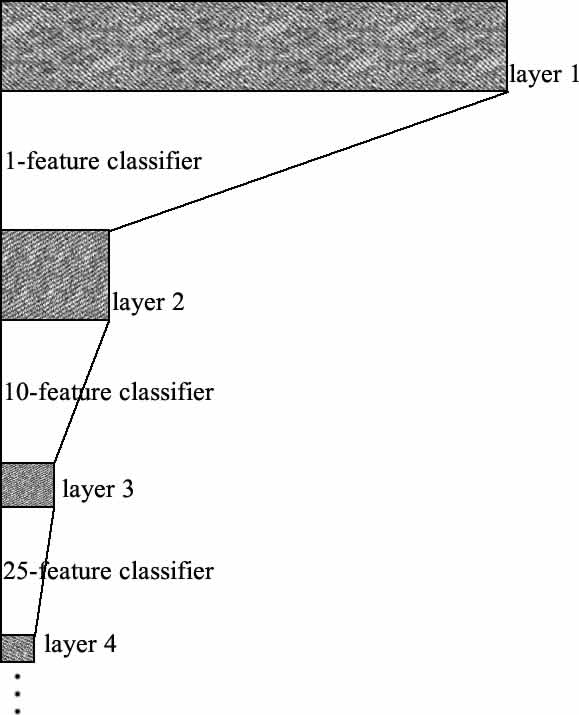
\includegraphics[width=0.8\linewidth]{cascading}
    \end{center}
    \caption{The cascading structure of the whole algorithm process. Data are picked from the original paper Section 5. Every classifier is trained under AdaBoost.}
    \label{fig:cs}
\end{figure}

\subsubsection{Selecting important features}
In selecting important features part, the authors used their previous work \cite{imgret}.
In that method, some features are firstly selected as highly selective features(HSF) which are based on their even previous work \cite{imgdb}.

HSF are a such set of features that they can respond to only a small percentage of images in the input (e.g. 5\%).
The respond in practical means applying convolutions between HSF and input can produce very large numerical values, and it is very efficient.
In the paper, such HSF are the important features.

Additionally, due to the rarity of those features, they use AdaBoost to select HSF.
For each weak learner in that AdaBoost, it computes a two class Gaussian model for the with-face images and non-face images,
and returns the feature for which the model is most sensitive. Figure \ref{fig:hsf} shows a set of HSF.

\begin{figure}[t]
    \begin{center}
        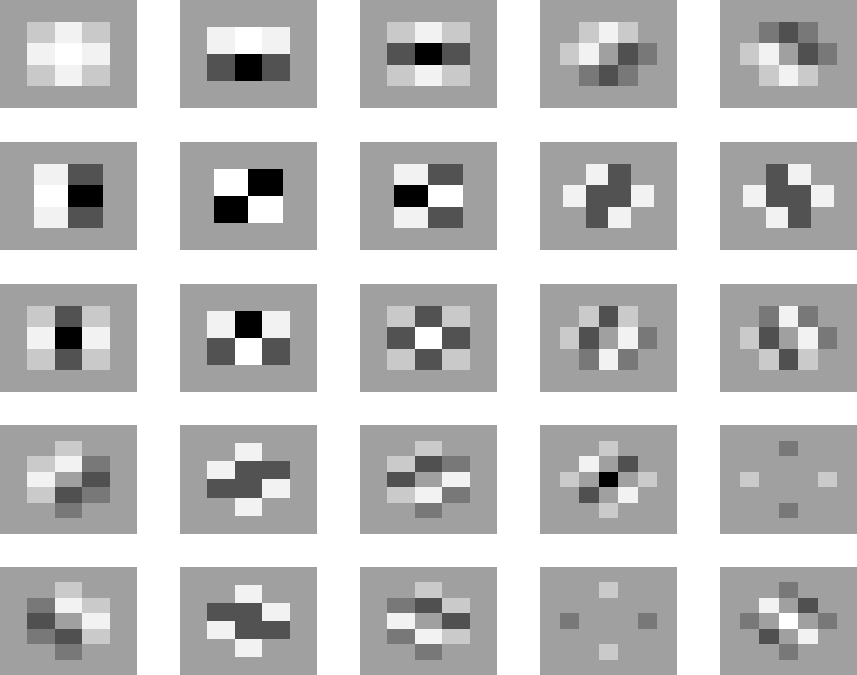
\includegraphics[width=0.9\linewidth]{highly-selective-features}
    \end{center}
    \caption{Sample highly selective features from Viola's previous paper \cite{imgret}.}
    \label{fig:hsf}
\end{figure}

\subsubsection{Constructing classifiers for selected features}
Foe each selected important features, we still don't know the relationship between them and the image classification.
That means, to separate the with-face images and non-face images perfectly, we need a threshold as the divider of the two kind of images.
They introduce the an important indicator of the resulting classifier - ``optimal threshold'', which can make sure that
when using a specific feature, minimum number of examples will be misclassified.
And, in each round of AdaBoost algorithm, only the most optimal threshold is selected for the weak classifier (weak learner).

In the paper, the weak learners are in this form:
\begin{equation}
\label{eq:hjx}
h_{j}(x)=\left\{\begin{matrix*}[l]
1 & \textup{when} \; p_{j}f_{j} < p_{j}\theta _{j}\\
0 & \textup{otherwise}
\end{matrix*}\right.
\end{equation}
where $h_{j}(x)$ is the $j$-th classifier among AdaBoost's final strong classifiers, and $x$ is a 24x24 pixel rectangle of an image.
$p_{j}$ is used to mark the positive (1, representing face) and negative (-1, representing non-face).
$f_{j}$ is a Haar-like features, and a threshold $\theta _{j}$ is used for best separating positive and negative features.

In the demonstration from the paper, all the 24x24 pixel rectangles are marked positive in a with-face image,
whereas all the 24x24 pixel rectangles are marked negative in a non-face image.
The error rates of the weak learners selected in early round can often achieve between 0.1 to 0.3 which is quite good.
However, when entering later rounds, the error rates increase to around 0.5, because the task gets more difficult.

Combining all the weak learners, the final classifier will be:
$$h(x)=\left\{\begin{matrix*}[l]
1 & \textup{when} \; \sum_{t=1}^{T} \alpha _{t} h_{t}(x) \geq \frac{1}{2} \sum_{t=1}^{T} \alpha _{t}\\
0 & \textup{otherwise}
\end{matrix*}\right.$$
where $\alpha _{t}$ is calculated by accumulated weighted error rate which is calculated during the procedure of selecting weak learners in AdaBoost algorithm.
$h_{i}(x)$ is the weak learner mentioned in Equation (\ref{eq:hjx}). $T$ is the total round number, which is also the number of weak learners.
In the paper, the number of $T$ is not mentioned, but in AdaBoost it's often a round counter,
and the choice of value depends on the prediction performance (which will be discussed in Section \ref{sec:hypo}).


\section{Hypothesis and Experiments} \label{sec:hypo}
To train the model is not feasible, due to the required data are super large. And the data I checked from famous institutions are testing data only.
Therefore I used the two pre-trained models from OpenCV directly \cite{opencvmodels},

\begin{itemize}
    \item \textbf{haarcascade\_frontalface\_default.xml}

          The default model for face detection with windows size (rectangle size) of 24x24, which is the same as what's mentioned in Viola and Jones's paper in 2001.
          The difference is this model is better than the 2001 year's one.

          I searched for plenty of websites, even checked the commit history of OpenCV documentation \cite{opencvdochistory}
          and the history of the model files \cite{opencvmodelhistory}, that model was just committed by a user named ``vpisarev'' in 2013.

    \item \textbf{haarcascade\_frontalface\_alt.xml}

          This is slightly different with the default model, the windows size here is 20x20. The detection results are different from the default model.

\end{itemize}

The overall performance of the pre-trained model with windows size of 24x24 are shown in Figure \ref{fig:overall}.
And only one face is not detected, the reason might be the combined disturbance of light and shading direction, skin colour and glasses on face.

\begin{figure}[t]
    \begin{center}
        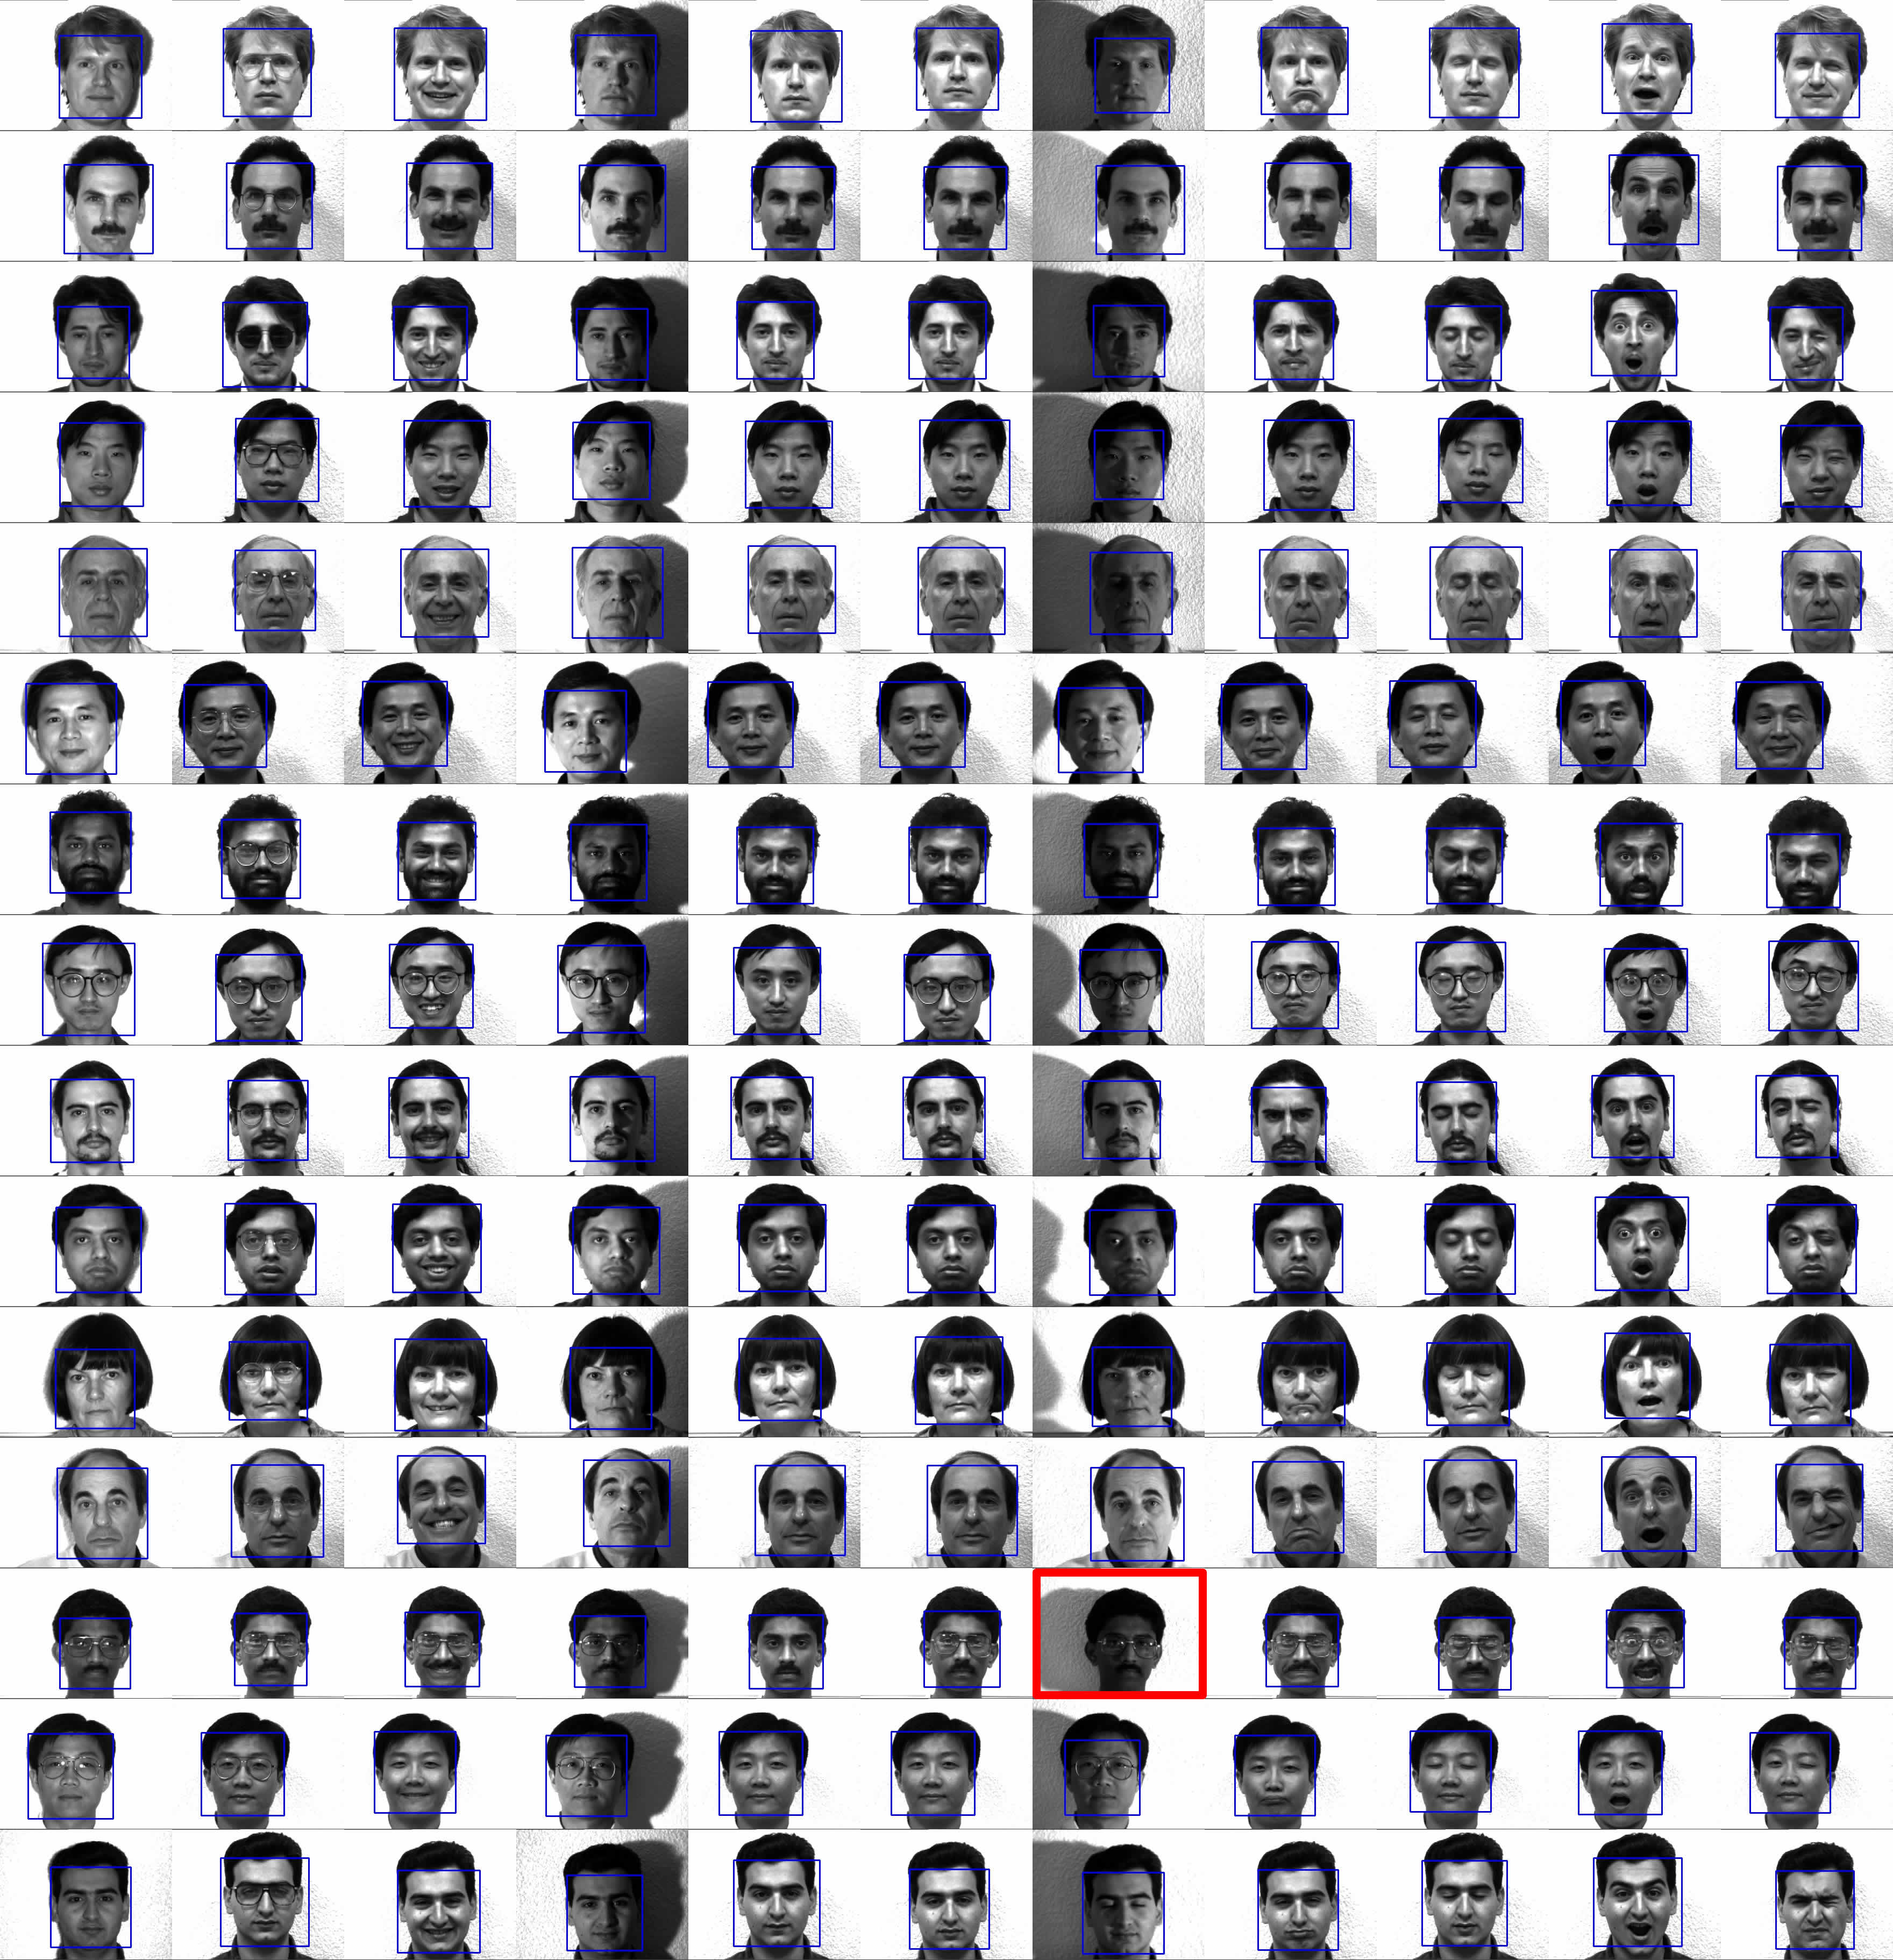
\includegraphics[width=0.9\linewidth]{yaleall}
    \end{center}
    \caption{Images from Yale database \cite{yaleimages} are all with size of 320x243, and only one face (marked in red) is not detected which might
    because the reason from light direction, skin colour and glasses.}
    \label{fig:overall}
\end{figure}


\subsection{Single feature performs bad}
In the partial demonstration in Section 3 of the original paper, the author showed that with 200 feature's classifier can achieve 95\% percent accurate.
However, in the cascading structure, the first layer contains only one feature during the final results from Viola and Jones's paper (Figure \ref{fig:cs}).

The authors already mention that no single feature can work perfectly, but the combination of selected features can works perfectly in Section 3.
However, for the best performance, it is very essential to use only one feature to filter the all the features.
In other words, the early layers are easy to be classified, unlike later layers which had to use lots features to classify accurately.
As a result, training AdaBoost to fit only one feature has a large probability to lead into over-fitting.

\subsection{Overfit causes problems}
AdaBoost can always overfit if the fit process keeps going on.
I believe selecting a proper maxima training round is very important, but the authors didn't mention the training details in the paper.

The authors show a receiver operating characteristic (ROC) curve (Figure 7 in original paper), which indicates that the more false positives are actually with higher correct detection rate.
This looks disobeying my hypothesis, but I think the $X$-axis showed only 200 false positives among 75 million sub-windows.
If the model is getting overfit, the number of false positives will get higher, whereas the correct detection rate will get dropped.

\subsection{Slicing step size, scaling step size and window size also affect the prediction result}
Voila and Jones mention that with smaller slicing step size or/and smaller scale step size, the accuracy can be improved for a certain degree.
Because the small step can capture more small features, and more difficult to lose small features.
But they didn't mention the different performance between different window size.

In my hypothesis, the smaller windows size is more sensitive to super small images.
OpenCV provides two pre-trained models with difference windows sizes: 20x20 and 24x24.
So, I tested them in very small images and proved in Figure \ref{fig:ysmall} and \ref{fig:yori}.
I also tested even smaller images, but none of the two models can detect any face in that images database.

\begin{figure}[t]
    \begin{center}
        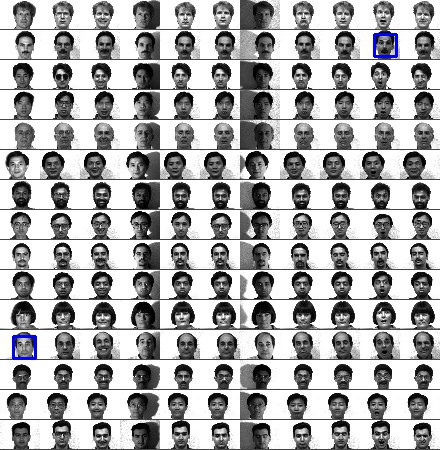
\includegraphics[width=0.9\linewidth]{yaleallsmall}
    \end{center}
    \caption{The images from Yale database are compressed into 40x30 size, and this is the results from 20x20 window size model. Two faces can be detected.}
    \label{fig:ysmall}
\end{figure}

\begin{figure}[t]
    \begin{center}
        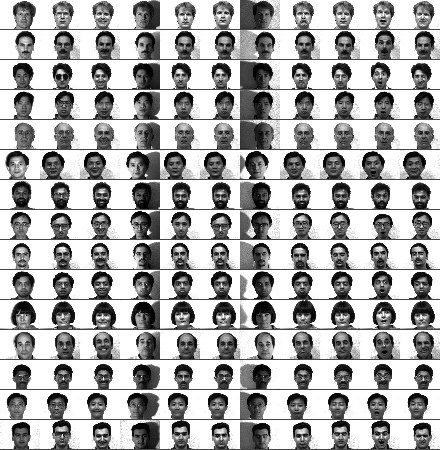
\includegraphics[width=0.9\linewidth]{yaleallsmall_ori}
    \end{center}
    \caption{The images from Yale database are compressed into 40x30 size, and this is the results from 24x24 window size model. None of the faces can be detected.}
    \label{fig:yori}
\end{figure}

Moreover, the smaller windows size are even more sensitive to the shade objects in face.
I tested the hair above one eye as the shades in Figure \ref{fig:hair}, the smaller windows size didn't detect the face.

\begin{figure*}
    \begin{center}
        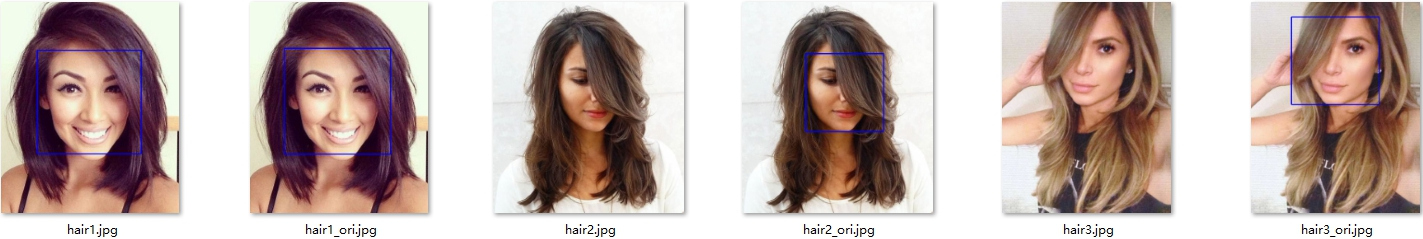
\includegraphics[width=0.9\textwidth]{hairstyle}
    \end{center}
    \caption{The smaller window size model performs worse when there are shading objects above face, here the shade is the hair.
    File names ended with ``\_ori'' are detected by 24x24 window size, with 3 of 3 images detected; the rest are by 20x20 small window size model, with 1 of 3 detected.}
    \label{fig:hair}
\end{figure*}

\subsection{Feature patterns are selected automatically}
The first features selected shown in the Figure 4 in original paper are around eyes and noses, where the eyes are darker than the bridge of the nose.
However, they are still automatically selected by AdaBoost, and it depends on the input data. The potential patterns like this are learnt by computer itself.
If the input images contains lots of faces of back skin, the first feature might not because eyes are darker than the bridge of the nose.

\subsection{The algorithm is multi-threading friendly}
In modern machine learning and computer vision area, multi-threading becomes more and more important due to the limitation of single CPU core.
In this algorithm, the features can be calculated simultaneously in different threads, because they are independent with each other.
When scanning the whole image, it can be divided into multiple block for multi-threading as well.

AdaBoost is not multi-threading friendly natively, because each round requires the previous round's result

\subsection{Training and predicting result is very stable}
The prediction result is very stable, using the same model to predict the same data will always get the same result.

The training process is also stable with the same configuration (step size, etc.),
because the model is a certain value calculated in the iterations of AdaBoost,
and this machine learning method does not use any randomized calculation.
Unlike other methods like Random Forest Classifier, using a random decision tree,
and each model are different with each other even with the same configuration.

\subsection{Model performance highly depends on training data}
In the motivation of this paper, any kind of face can be detected if the training data are provided.
The normal concerns are facial expressions, face decorations and etc., for training based algorithms, it require more variant input images to come over this.
Therefore, for the training data, if we giving 10,000 images marked as an object, and many images marked as not an object,
the resulting model should be able to detect that object from the input testing data.

A more specific example, by Voila and Jones, they trained the model with more than 10,000 marked images of frontal faces.
That means, if the face in images is not frontal or the face is tilted, the model cannot detect it. (See Figure \ref{fig:tilt} and Figure \ref{fig:tiltcor}.)

\begin{figure}[t]
    \begin{center}
        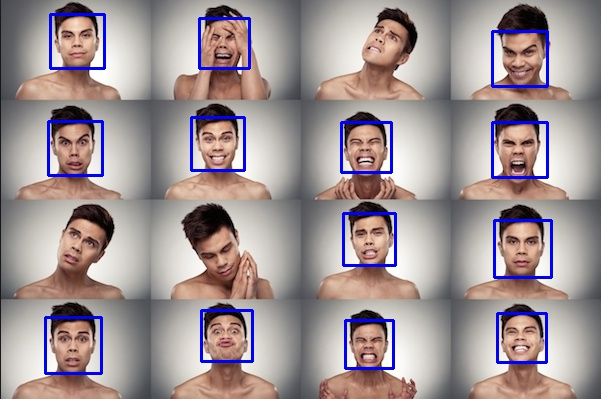
\includegraphics[width=0.9\linewidth]{facial1}
    \end{center}
    \caption{The image containing tilted faces examined with modelled trained without tilted faces. This image is from random search \cite{facialimg}.}
    \label{fig:tilt}
\end{figure}

\begin{figure}[t]
    \begin{center}
        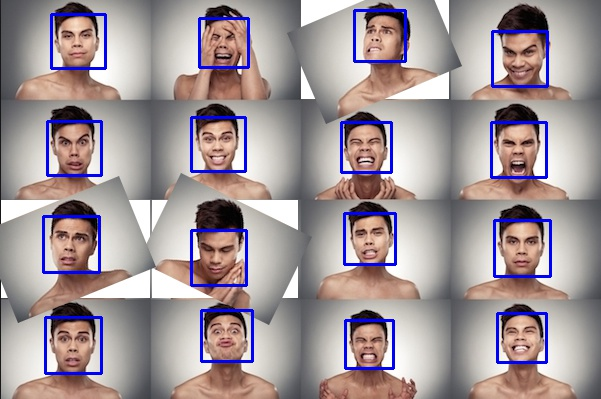
\includegraphics[width=0.9\linewidth]{facial1_corrected}
    \end{center}
    \caption{The corrected predicting result, this proves that the facial expression is not the reason of not being detected.}
    \label{fig:tiltcor}
\end{figure}

To come over this, the training image data set should contain lots of tilted faces to some extend.

\subsection{Haar-like features are very unstable for image noises}
At the beginning, I think the Haar-like features are not sensitive to the noises in images,
because the features use the sum of pixels, and noises are more like random added.
Therefore, the accumulated value of random numbers should have very little impacts on the final sum.
I did the experiment with coloured noises and grey noises (see Figure \ref{fig:noise}), it showed the noise still have some certain impacts on the images.

\begin{figure*}
    \begin{center}
        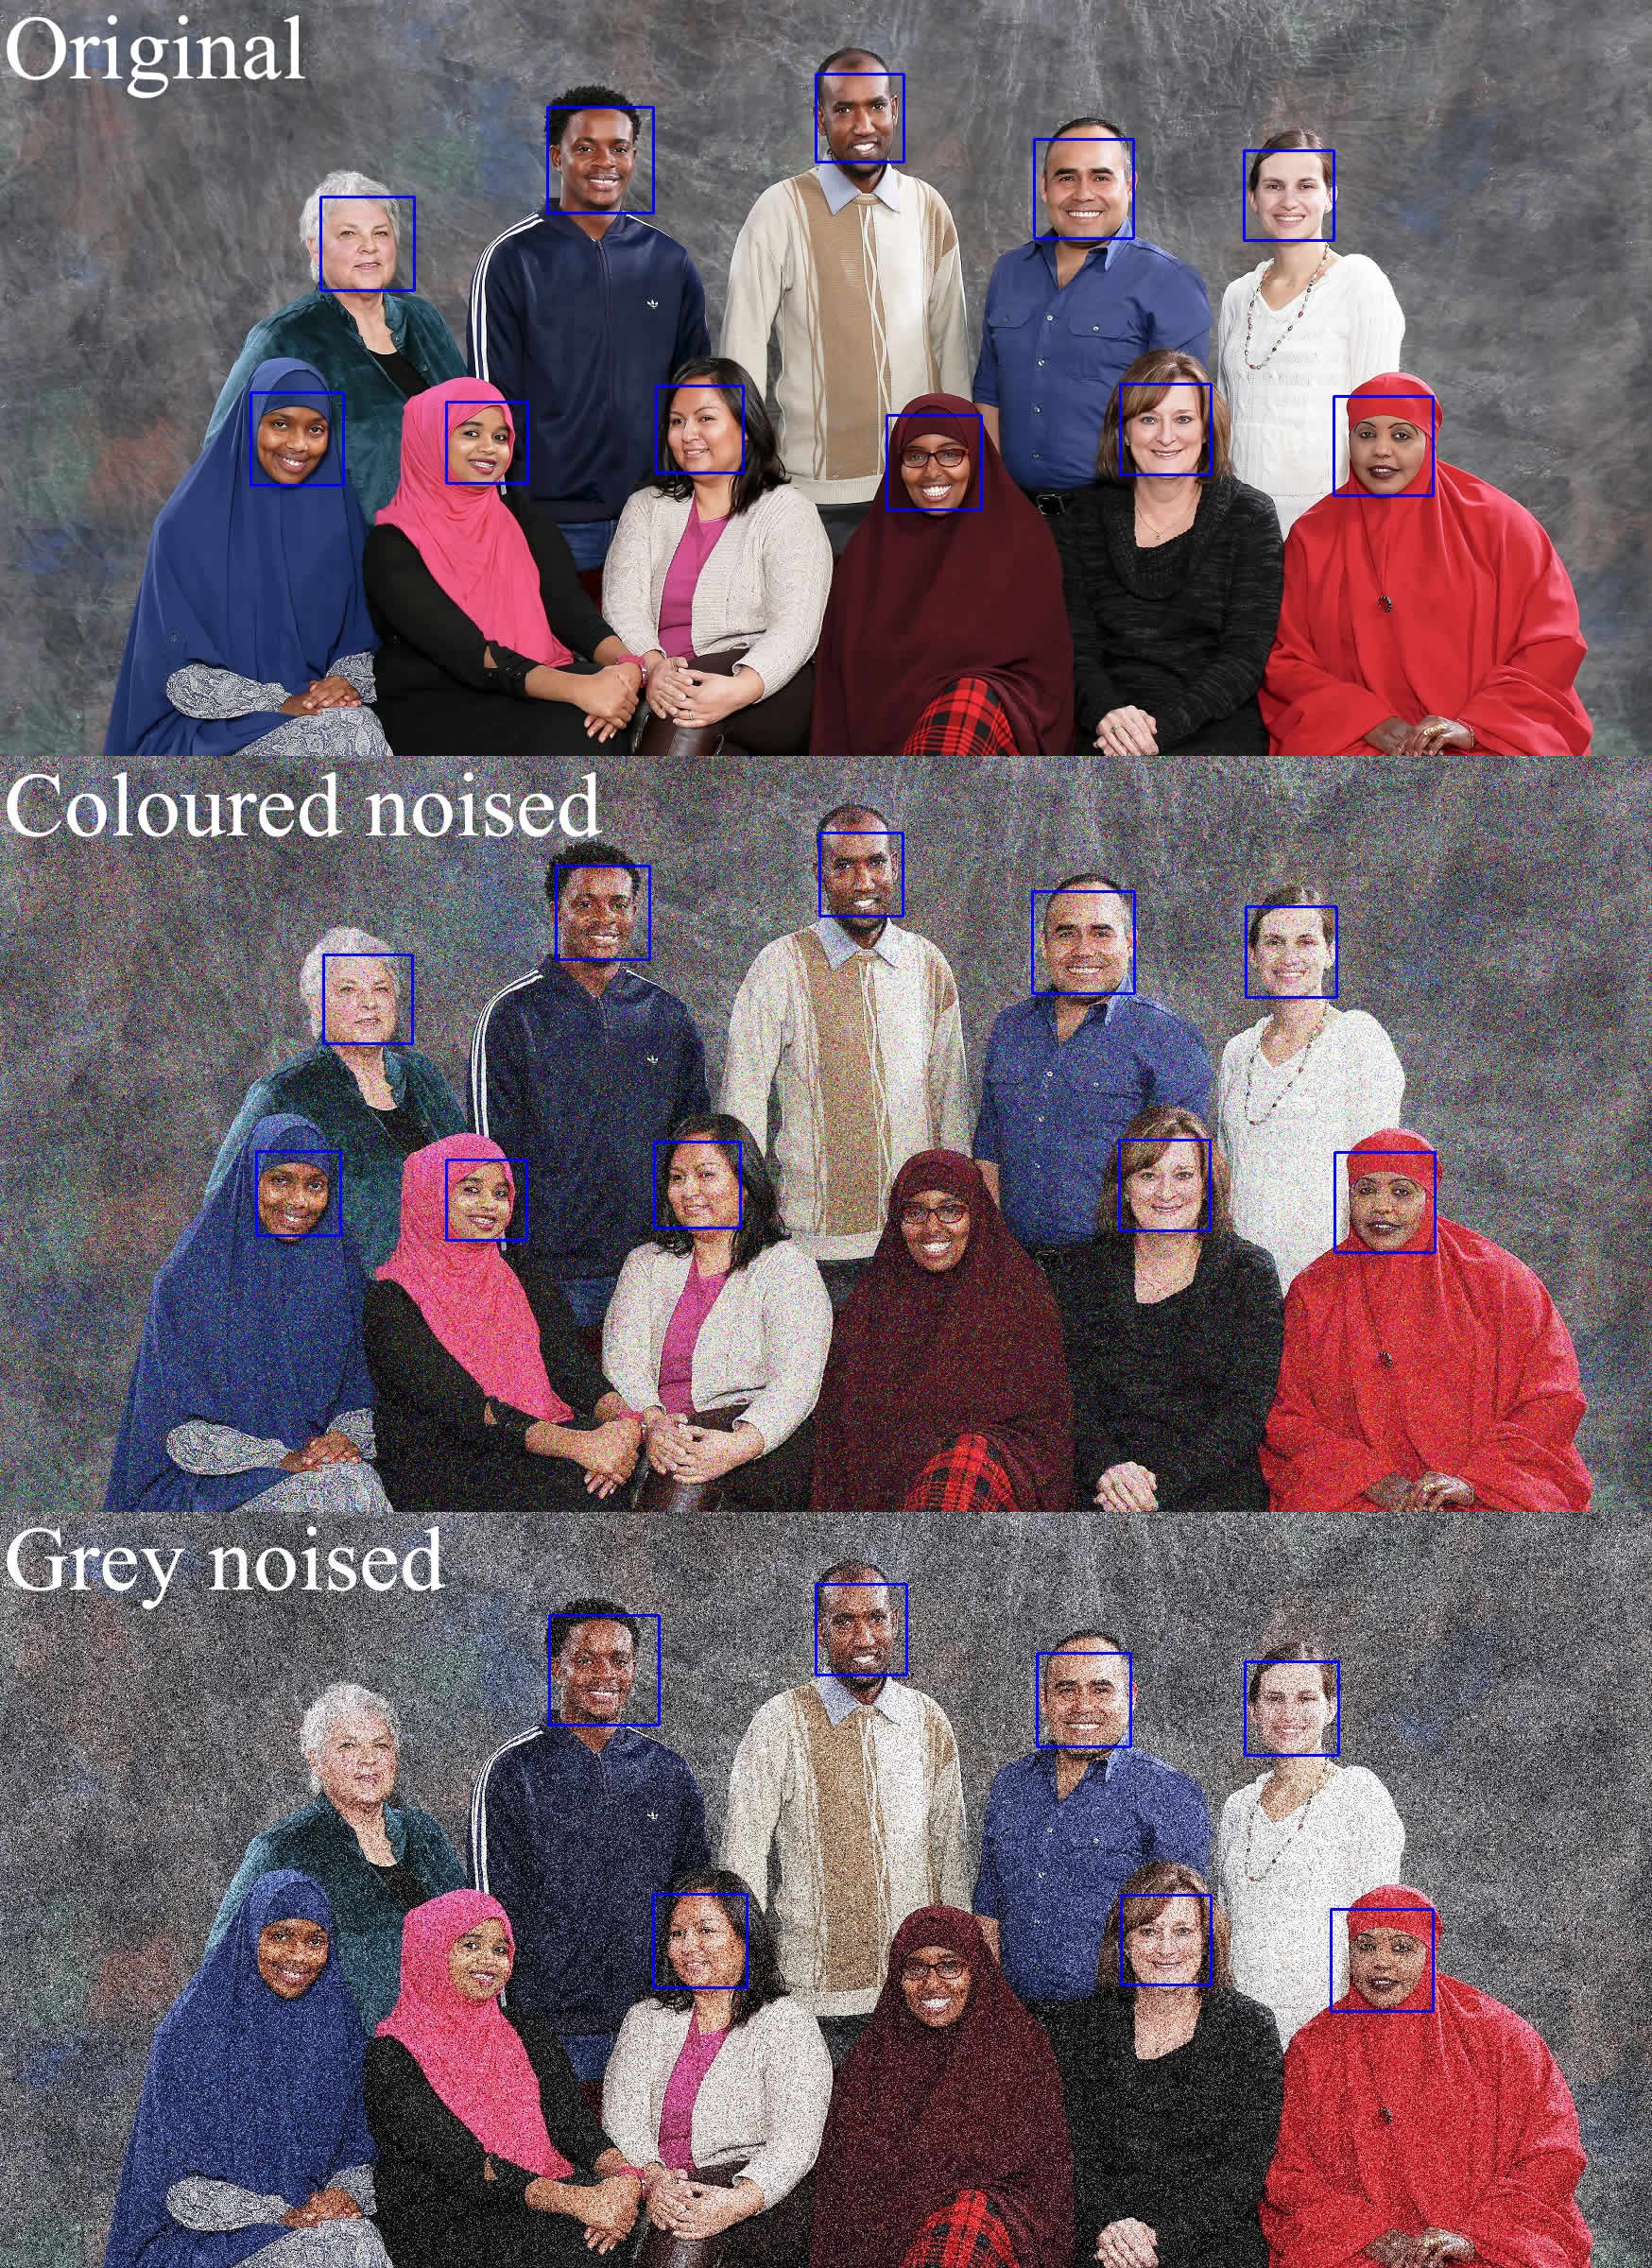
\includegraphics[width=0.9\textwidth]{11people-noised}
    \end{center}
    \caption{The noises \cite{noise} have significant bad impacts \cite{skinface} on the algorithm.}
    \label{fig:noise}
\end{figure*}

After this experiment, I think the reason might be the selected features have very high contrasts.
And noised images cannot provide very apparent contrasts for the model.
As a result, the Haar-like features are still sensitive to image noises.


\section{Conclusion and extensions}
In 2001, this algorithm can outperform other approaches 15 more times, and with nowadays computational ability,
it must be able to perform better using a smaller window size and smaller slicing/scaling step sizes.
And this will achieve a more accurate detecting rate.

As is mentioned in the introduction section in the original paper, some video face detection methods can outperform their algorithm.
Because in video, the images are continuous, so the difference between adjacent frames can be used directly for reducing computing time.

However, the authors didn't refer to any kind of video face detection papers.
I thought a very simple but efficient algorithm to calculate the difference between the two images - using mask to
calculate the absolute difference between the adjacent two frames (for example, see Figure \ref{fig:ext}).

\begin{figure}[t]
    \begin{center}
        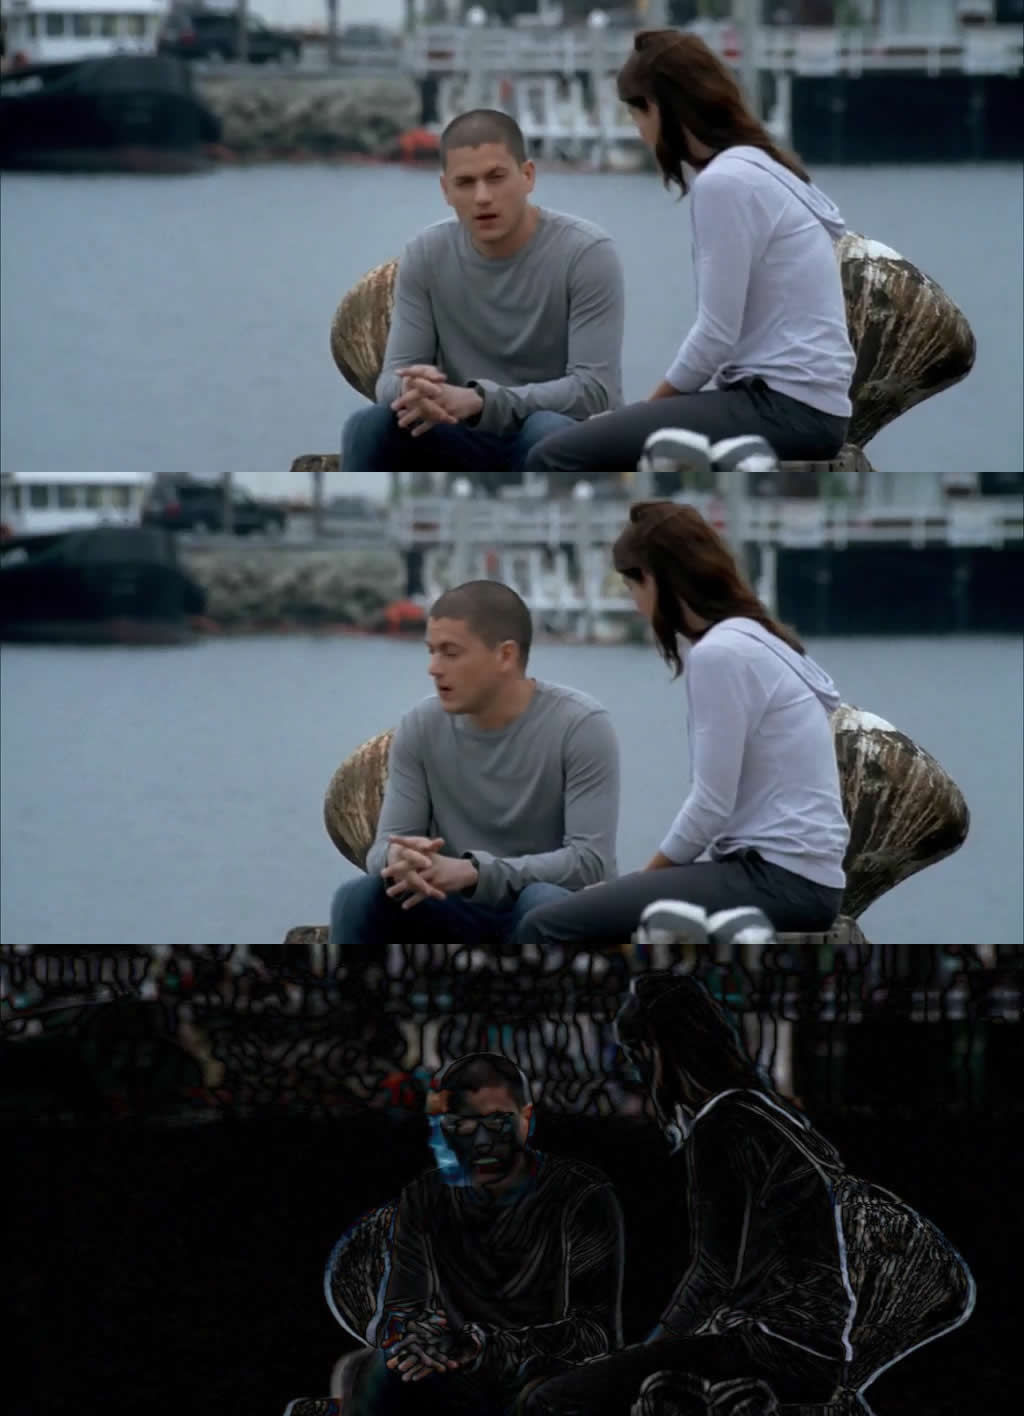
\includegraphics[width=0.9\linewidth]{extension}
    \end{center}
    \caption{The first two images are adjacent frames picked randomly from \textit{Prison Break S4E04 1:32},
    the first image is the second image's mask to produce the third image.
    The marks in the third images indicates which layer are the features discarded in selected areas in the cascading structure.}
    \label{fig:ext}
\end{figure}

Initially, current frame should be marked like the third picture in Figure \ref{fig:ext} by Viola and Jones' method,
and the main idea is to find the ``different areas'' between the two frames but with higher layer numbers.
I call it high probable areas.
Then re-calculate those areas with ``high difference'' only, to detect the potential faces.
The ``high difference'' threshold might also be learnt from AdaBoost.

Voila and Jones's works showed that AdaBoost was quite powerful than I expected.
And by machine learning methods, the potential patterns can be automatically and easily found,
the only challenge is to reduce the computational cost.
Moreover, the face detection algorithm is the basis of face recognition area,
and lots of object detection works are based on Viola and Jones's work which is quite impressive.


% Bibliography
\begin{thebibliography}{99}
\bibitem {origin}
P. Viola and M. Jones, ``Rapid object detection using a boosted cascade of simple features,''
In \textit{Proc. IEEE Conf. Comput. Vis. Pattern Recog.}, 2001, pp. 511–518.

\bibitem {adaboost}
Y. Freund and R.E. Schapire, ``A decision-theoretic generalization of online learning and an application to boosting,''
In \textit{Computational Learning Theory: Eurocolt '95}, pages 23-27, Springer-Verlag, 1995.

\bibitem {joint}
Y. Amit, D. Geman, and K. Wilder, ``Joint induction of shape features and tree classfiers,'' 1977.

\bibitem {snowbased}
D. Roth, M. Yang, and N. Ahuja, ``A snowbased face detector,''
In \textit{Neural Information Processing 12}, 2000.

\bibitem {nnbased}
H. Rowley, S. Baluja, and T. Kanade, ``Neural network-based face detection,''
In \textit{IEEE Patt. Anal. Mach. Intell.}, volume 20, pages 22-38, 1998.

\bibitem {stat3d}
H. Schneiderman and T.Kanade, ``A statistical method for 3D object detection applied to faces and cars,''
In \textit{Inernational Conference on Computer Vission}, 2000.

\bibitem {examplebased}
K. Sung and T. Poggio, ``Example-based learning for view-based face detection,''
In \textit{IEEE Patt. Anal. Mach. Intell.}, volume 20, pages 39-51, 1998.

\bibitem {imgret}
K. Tieu and P. Viola, ``Boosting image retrieval,''
In \textit{Proceedings of the IEEE Conference on Computer Vision and Pattern Recognition}, 2000.

\bibitem {imgdb}
J. S. DeBonet and P. Viola, ``Structure driven image database retrieval,''
In \textit{Adv. Neur. Info. Proc. Sys.}, volume 10, 1998.

\bibitem {opencvmodels}
opencv/data/haarcascades at master - opencv/opencv,
\url{https://github.com/opencv/opencv/tree/master/data/haarcascades}

\bibitem {opencvdochistory}
History for doc - opencv/opencv,
\url{https://github.com/opencv/opencv/commits/master/doc}

\bibitem {opencvmodelhistory}
History for data/haarcascades - opencv/opencv,
\url{https://github.com/opencv/opencv/commits/master/data/haarcascades}

\bibitem {yaleimages}
Yale Face Database,
\url{http://vision.ucsd.edu/content/yale-face-database}

\bibitem {facialimg}
These Amazing Photo Collages Display The Wide Range Of Human Emotions! Awesome Work!,
\url{http://www.viralspell.com/amazing-photo-collages-display-wide-range-human-emotions-awesome-work/}

\bibitem {skinface}
Blue Cross' Community Table aims to improve health for Willmar's increasingly older and more diverse community,
\url{https://blog.bluecrossmn.com/future-face-minnesota-look-willmar/}

\bibitem {noise}
Add noise online,
\url{http://pinetools.com/add-noise-image}

\end{thebibliography}

\end{document}
